\section{Graphen}



%Abstract FEHLT

\subsection{Begriffe}

Ein Graph ist eine abstrakte Struktur, die eine Menge von Objekten zusammen mit den zwischen diesen Objekten bestehenden Verbindungen repräsentiert. 

Die Objekte werden dabei \textbf{Knoten} des Graphen genannt. 
Die paarweisen Verbindungen zwischen Knoten heissen \textbf{Kanten}. 
Die Kanten können \textbf{gerichtet} oder \textbf{ungerichtet} sein, wenn die Verbindungen zwischen den Knoten, eine Richtung beinhalten (oder nicht).

Am einfachsten kann man Graphen zeichen, indem Knoten durch Punkte und die Kanten durch Linien (ungerichtet) oder durch Pfeile im gerichteten Fall darstellt. 

\begin{mbsp}
%\paragraph{Beispiel:}
Anschauliche Beispiele für Graphen sind ein Stammbaum oder das S-Bahn-Netz (s. Abb.~\ref{fig:sbahn}) einer Stadt. 
Bei einem Stammbaum stellt jeder Knoten ein Familienmitglied dar und jede Kante ist eine Verbindung zwischen einem Elternteil und einem Kind. 
In einem S-Bahn-Netz stellt jeder Knoten eine S-Bahn-Station dar und jede Kante eine direkte Zugverbindung zwischen zwei Stationen.
\end{mbsp}
%\begin{figure}[htb]
%\begin{center}
%
%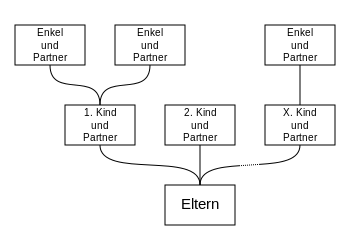
\includegraphics[width=.67\textwidth]{../fig/stammbaum.png}
%%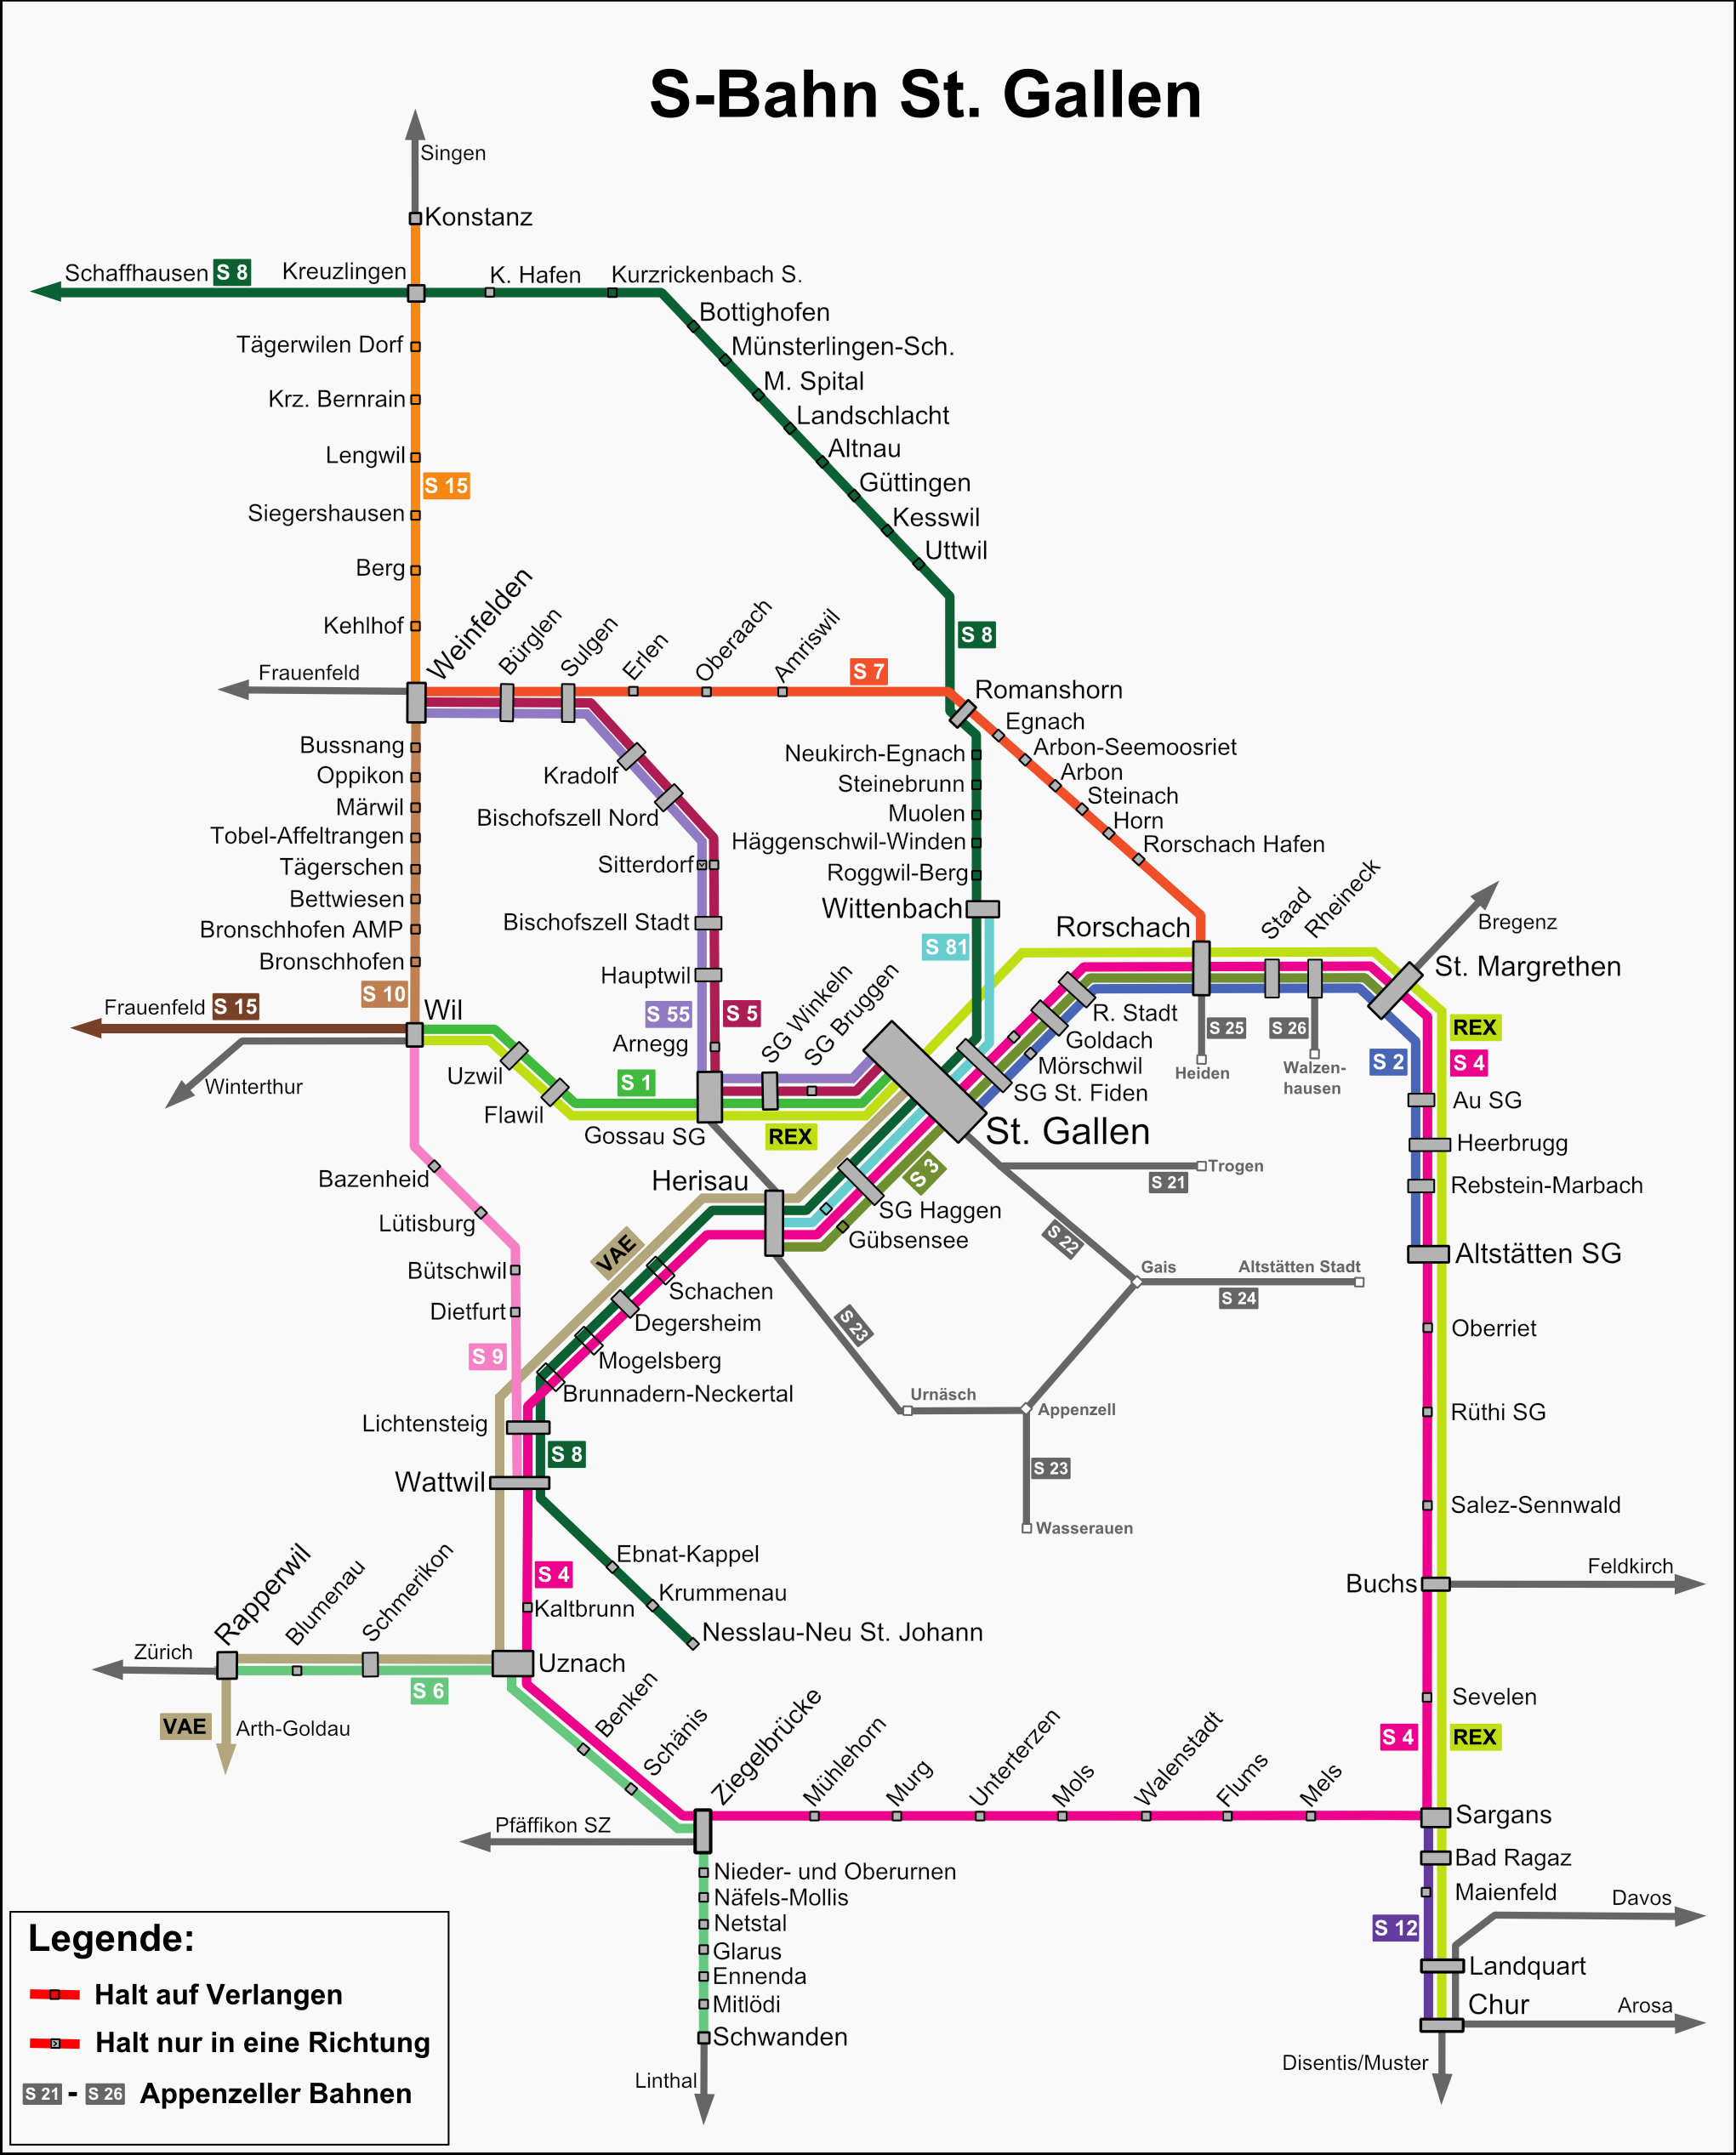
\includegraphics[width=.45\textwidth]{../fig/sbahn_netz.png}
%\caption{Darstellung eines Stammbaumes als (ungerichteter) Graph.
%Jedes Familienmitglied (Enkel, Kind, Eltern) ist ein Knoten und die Kanten bilden die Verbindungen zwischen Eltern und Kindern.
%%https://upload.wikimedia.org/wikipedia/commons/thumb/c/c1/Stammbaum.svg/400px-Stammbaum.svg.png
%}
%\label{fig:stammbaum}
%
%\end{center}
%\end{figure}

\begin{figure}[htb]
\begin{center}

%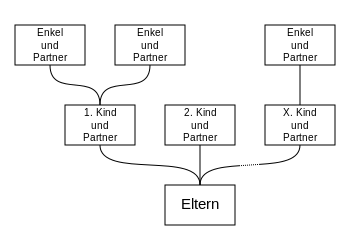
\includegraphics[width=.7\textwidth]{../fig/stammbaum.png}
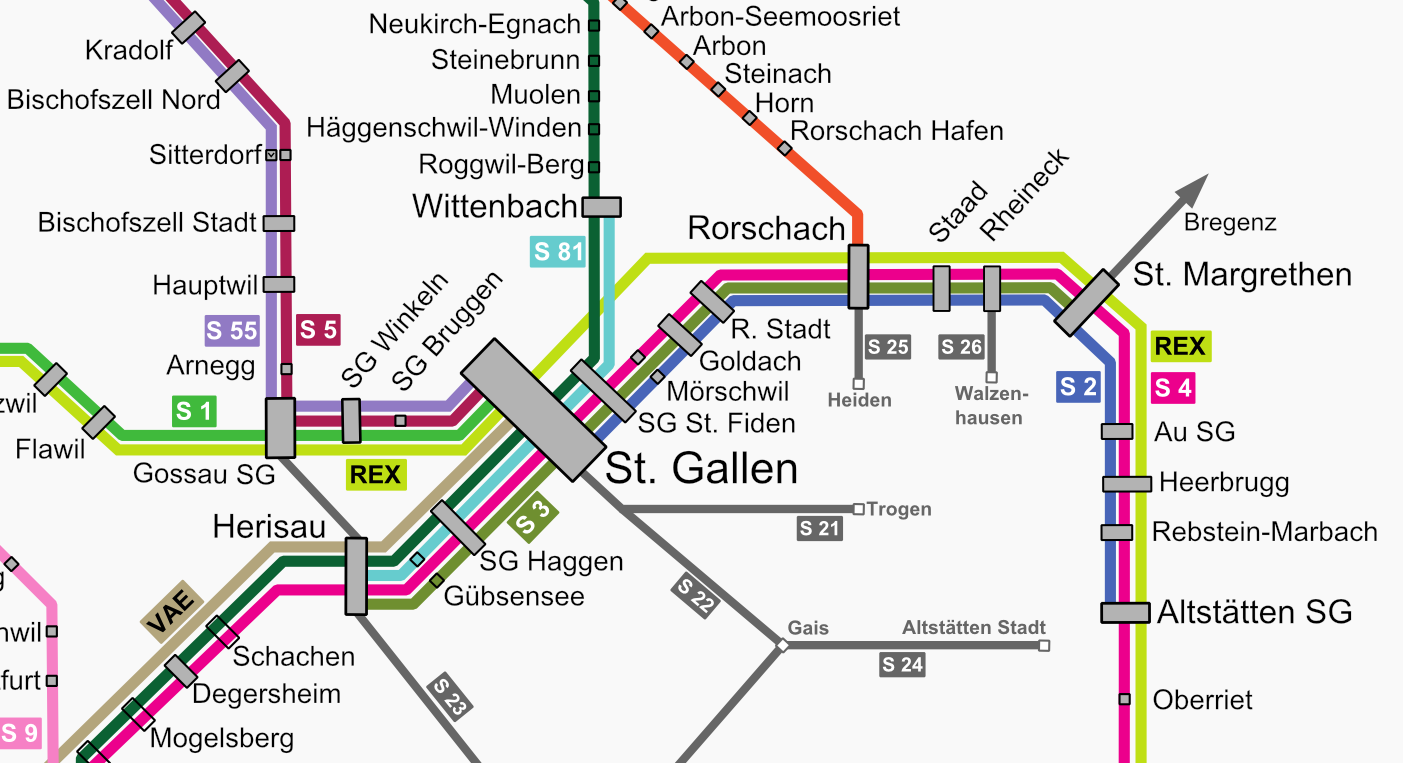
\includegraphics[width=.67\textwidth]{../fig/sbahn_netz_ausschnitt.png}
\caption{Darstellung eines Ausschnitts des Sankt Galler S-Bahn-Netzes als (ungerichteter) Graph.
Jede Station bildet dabei einen Knoten und die Verbindung zwischen den Knoten ist eine Kante.
%https://upload.wikimedia.org/wikipedia/commons/1/19/Map_S-Bahn_St._Gallen_%28schematic%29.png
}

\label{fig:sbahn}
\end{center}
\end{figure}


\subsection{Defintionen}

\begin{mdef}
%\paragraph{Graph:}
Mathematisch besteht ein \textbf{Graph} $G$ aus einer \textbf{Menge} von \textbf{Knoten} $V$ (engl. \emph{vertex}) und einer \textbf{Menge} von \textbf{Kanten} $E$ (engl. \emph{Edge}).
Die Anzahl Knoten wird mit $|V|$ und die Anzahl Kanten mit $|E|$ bezeichnet.
\end{mdef}



\begin{mdef}
%\paragraph{Ungerichteter Graph:}
Jede Kante eines \textbf{ungerichteten Graphen} $e$ besteht aus zwei Knoten $v_1$ und $v_2$ und wird selbst als Menge dargestellt: $e= \{v_1,v_2\}$.
Die Reihenfolge spielt dabei keine Rolle: $\{v_1,v_2\} = \{v_2,v_1\}$.
\end{mdef}

\begin{mdef}
%\paragraph{Gerichteter Graph:}
Jede Kante eines \textbf{gerichteten Graphen} $e$ besteht aus einem Startknoten $v_1$ und einem Zielknoten $v_2$ und wird selbst als 2-Tupel dargestellt: $e= (v_1,v_2)$. 
Hierbei spielt die Reihenfolge ein Rolle: $(v_1,v_2) \neq (v_2,v_1)$. 
\end{mdef}


\begin{mbsp}
%\paragraph{Beispiele:}
Die Abblidung~\ref{fig:bsp:ugraph} zeigt einen ungerichteten Graph mit 5 Knoten und einen gerichteten Graphen mit 6 Knoten. 
\end{mbsp}

\begin{figure}[htb]
\begin{center}
\begin{tikzpicture}[-,>=stealth',shorten >=1pt,auto,node distance=2.8cm,
                    semithick, style=circle]
  \tikzstyle{wstate}=[fill=white,text=black,draw=black]
%  \tikzstyle{gstate}=[fill=gray,text=black,draw=black]
%  \tikzstyle{bstate}=[fill=black,text=white,draw=black]
  

  \node[wstate]         (1) 			 {$1$};
    \node[wstate] 		(0) [below of=1] {$0$};
  \node[wstate]         (2) [right of=1] {$2$};
  \node[wstate]         (3) [below right of=2] {$3$};
  \node[wstate]         (4) [below of=2]       {$4$};
%  \node[wstate]         (2) [above right of=4]       {$2$};

  \path (0) edge              node {} (1)
            edge              node {} (2)
            edge              node {} (4)
        (1) edge 			  node {} (2)
        (3) edge              node {} (2)
	        edge  			  node {} (4)
        (2) edge 			  node {} (4);
%            edge              node {} (4)
%        (4) edge [bend left]  node {} (0);
\end{tikzpicture}\hfill
\begin{tikzpicture}[->,>=stealth',shorten >=1pt,auto,node distance=2.8cm,
                    semithick, style=circle]
  \tikzstyle{wstate}=[fill=white,text=black,draw=black]
%  \tikzstyle{gstate}=[fill=gray,text=black,draw=black]
%  \tikzstyle{bstate}=[fill=black,text=white,draw=black]
  

  \node[wstate]         (1) 			 		{$1$};
  \node[wstate]         (2) [right of=1]		{$2$};
  \node[wstate]         (3) [right of=2]		{$3$};
  \node[wstate]         (4) [below of=1]		{$4$};
  \node[wstate]         (5) [right of=4]		{$2$};
  \node[wstate] 		(0) [right of=5]		{$0$};

  \path (0) edge	[loop right]	node {} (0)
        (1) edge 					node {} (2)
        	edge 					node {} (4)
        (2) edge            		node {} (5)
        (3) edge 					node {} (5)
        	edge					node {} (0)
        (4) edge   					node {} (2)
        (5) edge   					node {} (4);
        %[bend left]
\end{tikzpicture}

\caption{\emph{Links:} Ein ungerichteter Graph mit 5 Knoten. 
\emph{Rechts:} Ein gerichteter Graph mit 6 Knoten.
}
\label{fig:bsp:ugraph}
\end{center}
\end{figure}



%\begin{figure}[htb]
%\begin{center}
%
%%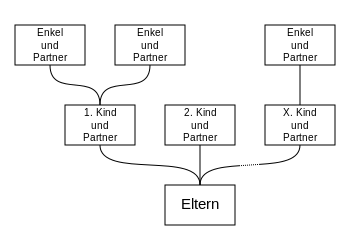
\includegraphics[width=.7\textwidth]{../fig/stammbaum.png}
%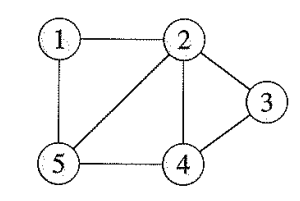
\includegraphics[width=.45\textwidth]{../fig/graph_ug_01.png}\hfill
%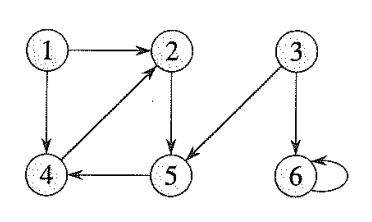
\includegraphics[width=.45\textwidth]{../fig/graph_ge_01.png}
%\caption{\emph{Links:} Ein ungerichteter Graph mit 5 Knoten. 
%\emph{Rechts:} Ein gerichteter Graph mit 6 Knoten.
%}
%\label{fig:bsp:ugraph}
%\end{center}
%\end{figure}

Die mathematische Darstellung der zwei Graphen lautet:

\[ \text{Graph links:} \quad G_l = (V_l, E_l); \quad V_l = \{0,1,2,3,4\}; \] 
\[\quad E_l =  \{ \{1,2\},\{1,0\},\{2,0\},\{2,4\},\{2,3\}, \{3,4\}, \{4,0\}. \}  \]

\[ \text{Graph rechts:} \quad G_r = (V_r, E_r); \quad V_r = \{0,1,2,3,4,5\}; \] 
\[\quad E_r =  \{ (1,2),(1,4), (2,5), (3,5), (3,0), (4,2), (5,4), (0,0)\}.  \]

\begin{aufg}
%\paragraph{Aufgabe:}
Bilden Sie für folgenden Graph (Abb.~\ref{fig:auf:graph}) die entsprechende mathematische Darstellung $G=(V,E)$.
\end{aufg}


\begin{figure}[htb]
\begin{center}
\begin{tikzpicture}[->,>=stealth',shorten >=1pt,auto,node distance=2.8cm,
                    semithick, style=circle]
  \tikzstyle{wstate}=[fill=white,text=black,draw=black]
%  \tikzstyle{gstate}=[fill=gray,text=black,draw=black]
%  \tikzstyle{bstate}=[fill=black,text=white,draw=black]
  
  \node[wstate] 		(0)                    {$0$};
  \node[wstate]         (1) [above of=0] {$1$};
  \node[wstate]         (2) [right of=1] {$2$};
  \node[wstate]         (3) [below right of=2] {$3$};
  \node[wstate]         (4) [below of=2]       {$4$};

  \path (0) edge              node {} (1)
            edge              node {} (2)
        (1) edge [loop above] node {} (1)
            edge              node {} (2)
        (3) edge              node {} (1)
            edge [bend left]  node {} (4)
        (2) edge [loop below] node {} (2)
            edge              node {} (0)
        (4) edge [bend left]  node {} (0);
\end{tikzpicture}
\caption{Ein gerichteter Graph.}
\label{fig:auf:graph}
\end{center}
\end{figure}


\begin{aufg}
%\paragraph{Aufgabe:} 
Zeichnen Sie den entsprechenden Graph, der zu folgender Mathematischen Darstellung gehört:

\[ \quad G = (V, E); \quad V = \{0,1,2,3,4,5,6\}; \] 
\[\quad E =  \{ (1,3),(1,6), (2,1), (3,3), (3,4), (4,2), (5,4), (6,3)\}. \]

\end{aufg}


\begin{mdef}
%\paragraph{Adjazenzmatrix:}
Für einen Graphen $G=(V,E)$ nehmen wir an, dass die Knoten in beliebiger Weise von 0 bis $|V|-1$ nummeriert sind.
So bildet die \textbf{Adjazenzmatrix-Darstellung} des Graphen $G$ eine $|V| \times |V|$-Matrix $A=a_{ij}$ mit den Elementen

\[ a_{ij} = 
  \begin{cases}
    1   & \quad \text{falls } (i,j) \in E, \\
   0   & \quad \text{sonst}
  \end{cases}.
\]

Für ungerichtete Graphen ersetzt man $(i,j) \text{ durch } \{i,j\}$.
\end{mdef}

\begin{mbsp}
%\paragraph{Beispiele:}
Die Adjazenz-Matrizen ($A_l$ und $A_r$) zu den zwei Graphen in Abb.~\ref{fig:bsp:ugraph} lauten:

\[ A_l =  \begin{pmatrix}
  0 & 1 & 0 & 0 & 1 \\
  1 & 0 & 1 & 1 & 1 \\
  0 & 1 & 0 & 1 & 0  \\
  0 & 1 & 1 & 0 & 1 \\
  1 & 1 & 0 & 1 & 0 \\
 \end{pmatrix};
\quad
A_r =  \begin{pmatrix}
  0 & 1 & 0 & 1 & 0 & 0 \\
  0 & 0 & 0 & 0 & 1 & 0 \\
  0 & 0 & 0 & 0 & 1 & 1 \\
  0 & 1 & 0 & 0 & 0 & 0 \\
  0 & 0 & 0 & 1 & 0 & 0 \\
  0 & 0 & 0 & 0 & 0 & 1 \\
 \end{pmatrix}.
  \]
\end{mbsp}

\begin{aufg}
%\paragraph{Aufgabe:} 
Bilden Sie für den Graphen aus Abbildung~\ref{fig:auf:graph} die entsprechende Adjazenzmatrix $G=(V,E)$.
\end{aufg}



\begin{aufg}
%\paragraph{Aufgabe:} 
Zeichnen Sie zu folgender Adjazenzmatrix den entsprechenden Graphen.


\[A =  \begin{pmatrix}
  1 & 1 & 0 & 0 & 1 & 0 \\
  0 & 0 & 1 & 0 & 1 & 0 \\
  0 & 1 & 0 & 0 & 1 & 1 \\
  1 & 0 & 0 & 0 & 0 & 0 \\
  0 & 1 & 0 & 1 & 1 & 0 \\
  0 & 0 & 1 & 0 & 1 & 0 \\
 \end{pmatrix}.
  \]
  
\end{aufg}

\begin{aufg}
%\paragraph{Programmierung:}
Damit man einen Graphen in einer Textdatei speichern und lesen kann, benutzt man häufig ';' (Semicolon) um die Zahlen einer Zeile zu trennen. 
Mit einem Absatz wird eine neue Zeile der Matrix bestimmt. 
Schreiben Sie ein Programm \textsc{NicePrint($graph$)}, dass die Adjazenzliste eines Graphen auf den Bildschirm ausgibt.
Benutzen Sie dafür das vorgegebene Programm, welches Graphen aus einer Textdatei einlesen kann und überprüfen Sie die Ausgabe mit den Textdateien.
\end{aufg}


\begin{mdef}
%\paragraph{Nachbarn:} 
Zwei Vertices sind zueinander \textbf{benachbart}, wenn eine direkte Verbindung durch eine Kante besteht. 
In einem ungerichteten Graphen sind immer beide Vertices benachbart. 
Hingegen spielt in einem gerichteten spielt die Richtung der Kante eine Rolle, so dass die Nachbarschaft nur in eine Richtung gelten kann.
\end{mdef}

\begin{mbsp}
%\paragraph{Beispiel:}
Im Graphen der Abbildung~\ref{fig:bsp:ugraph} links hat der Knoten 2 die Nachbarn 1,5,4 und 3. 
Dies kann man auch aus der Adjazenzmatrix $A_l$ ablesen: Die zweite Reihe hat dort bei den Spalten 1,3,4 und 5 eine eins stehen.

Im Gegensatz dazu hat der Knoten 2 im Graphen der Abbildung~\ref{fig:bsp:ugraph} rechts nur den Nachbarknoten 5. 
Auch dies kann man wieder aus der zweiten Reihe der Adjazenzmatrix $A_r$ ablesen.
\end{mbsp}

\begin{aufg}
%\paragraph{Aufgabe:} 
Welche Nachbarn hat der Knoten 3, der Knoten 1 und der Knoten 0 des Graphen in Abbildung~\ref{fig:auf:graph}.
\end{aufg}


\begin{aufg}
%\paragraph{Programmierung:}
Implementieren Sie eine Funktion \textsc{Nachbarknoten($graph$, $knoten$)}: Sie hat als Input einen Graphen und einen Knoten und gibt als Output eine Liste von Nachbarknoten des Knotens im Graphen aus. Testen Sie die Funktion, indem Sie sie mit verschiedenen Knoten aus einem Graphen aufrufen.
\end{aufg}

\subsection{Zusammenfassung und Kontrollaufgaben}

In diesem Kapitel haben Sie die Darstellung von Graphen wiederholt. 
Insbesondere haben Sie verschiedene Darstellung der Graphen kennen gelernt: Zeichnung, Menge von Kanten und Knoten und Adjazenzmatrix.
Zusätzlich kennen Sie den Unterschied zwischen gerichteten und ungerichteten Graphen und können die Nachbarn eines Knoten in einem Graphen bestimmen. 


%\subsection{Kontrollaufgaben}

%\begin{enumerate}
\begin{kontr}
Beschreiben Sie Unterschiede und Gemeinsamkeiten von gerichteten und ungerichteten Graphen.
\end{kontr}


\begin{kontr}
Nennen Sie drei weitere Beispiele aus dem Alltag für Graphen. 
Bestimmen Sie dabei immer was die Knoten und was die Kanten darstellen. 
Handelt es sich dabei um gerichtete oder ungerichtete Graphen?
\end{kontr}


\begin{kontr}
Betrachten Sie folgenden Graphen (s. Abb.~\ref{fig:kont:graph}) und bestimmen Sie seine Knoten und Kanten Menge und bestimmen Sie zusätzlich die Adjazenzmatrix.

\begin{figure}[htb]
\begin{center}
\begin{tikzpicture}[->,>=stealth',shorten >=1pt,auto,node distance=2.8cm,
                    semithick, style=circle]
  \tikzstyle{wstate}=[fill=white,text=black,draw=black]
%  \tikzstyle{gstate}=[fill=gray,text=black,draw=black]
%  \tikzstyle{bstate}=[fill=black,text=white,draw=black]
  
  \node[wstate] 		(0)                    {$0$};
  \node[wstate]         (3) [above of=0] {$3$};
  \node[wstate]         (4) [left of=0] {$4$};
  \node[wstate]         (1) [below right of=2] {$1$};
  \node[wstate]         (5) [below of=2]       {$5$};
  \node[wstate]         (2) [above right of=4]       {$2$};

  \path (0) edge              node {} (1)
            edge              node {} (2)
        (1) edge [loop right] node {} (1)
            edge              node {} (2)
        (3) edge              node {} (1)
      %      edge [bend left]  node {} (4)
        (2) edge [loop above] node {} (2)
            edge              node {} (4)
        (4) edge [bend left]  node {} (0);
\end{tikzpicture}
\caption{Ein weiterer Graph.}
\label{fig:kont:graph}
\end{center}
\end{figure}

\end{kontr}

\begin{kontr}
Betrachten Sie folgende Knoten- und Kantenmenge. Zeichnen Sie den dazugehörigen Graphen und Bestimmen Sie die dazugehörige Adjazenzmatrix.

\[ \quad G = (V, E); \quad V = \{2,3,4,5,6,7,9\}; \] 
\[\quad E =  \{ \{7,3\},\{9,6\}, \{2,6\}, \{3,2\}, \{3,4\}, \{4,2\}, \{5,4\}, \{7,9\}\}. \]

\end{kontr}

\begin{kontr}
Betrachten Sie folgende Adjazenzmatrix, zeichnen Sie den dazugehörigen Graphen und bestimmen Sie die Knoten- und Kantenmenge.

\[A =  \begin{pmatrix}
  0 & 1 & 0 & 1 & 1 & 0 \\
  1 & 0 & 1 & 0 & 1 & 0 \\
  0 & 1 & 0 & 0 & 1 & 1 \\
  1 & 0 & 0 & 0 & 0 & 0 \\
  1 & 1 & 1 & 0 & 0 & 1 \\
  0 & 0 & 1 & 0 & 1 & 0 \\
 \end{pmatrix}
  \]
\end{kontr}

%\end{enumerate}
